\documentclass[12pt]{article}

\usepackage[utf8]{inputenc}
\usepackage{enumitem}
\usepackage{dsfont}
\usepackage{hyperref}
\usepackage{listings}
\usepackage{xcolor}
\usepackage{graphicx}

\pagenumbering{arabic}

\definecolor{dkgreen}{rgb}{0,.6,0}
\definecolor{dkblue}{rgb}{0,0,.6}
\definecolor{dkyellow}{cmyk}{0,0,.8,.3}

\lstset{
  language        = php,
  basicstyle      = \small\ttfamily,
  keywordstyle    = \color{dkblue},
  stringstyle     = \color{red},
  identifierstyle = \color{dkgreen},
  commentstyle    = \color{gray},
  emph            =[1]{php},
  emphstyle       =[1]\color{black},
  emph            =[2]{if,and,or,else},
  emphstyle       =[2]\color{dkyellow},
  breaklines=true,
  postbreak=\raisebox{0ex}[0ex][0ex]{\ensuremath{\color{red}\hookrightarrow\space}}}

\title{Report - Mathematical expression as new data type for WikiData\\
Database project - Technical University Berlin}

\date{\today}
\author{Duc Linh Tran\\ Technische Universität Berlin\\ duc.l.tran@campus.tu-berlin.de
       \and Julian Hilbig\\ Technische Universität Berlin\\ julian.hilbig@campus.tu-berlin.de}


\begin{document}
\maketitle

\section{Abstract}
%Goal, Problem, Solution
Since 2001, Wikipedia is providing people around the world with information written by volunteers around the world, making Wikipedia the first  free-as-in-freedom online encyclopedia in more than 200 languages. Over time, Wikipedia evolved to distribute the information more efficient. One of the improvements is Wikidata, a database to unify and centralize language independent information. Currently, the content of each article about the same topic in a different language is independently written and edited. To provide similar kind of information more advanced options, like distance calculation for geographic coordinates, data types were created for WikiData. There is no data type for mathematical formula yet though, as on the one hand, mathematical formulae fulfill the requirements to have a data type in Wikidata and on the other hand, their properties do not match to already implemented data types. In our project as part of the "DBPRO: Datenbankprojekt" course of the Technical University Berlin, we define and implement this new data type for mathematical expressions and formulae.

\section{Introduction}
\paragraph{}
The WikiData project was launched in October 2012 by the Wikimedia Foundation with the goal to centralize and unify language independent information such as population of a city in a well structured database. %It is mainly supervised by Wikimedia Deutschland.
%TODO: citation needed
%TODO: call that datatypes that will make it clear to the target audience
There are many kind of information with similar traits for different properties. Therefore several data types were implemented. Examples are "monolingual text" for language independent words like names or "time" for birthdays or other specific dates. These add more use cases for the data than just raw information storage. There was not a fitting one for mathematical expressions though\footnote{Discussion about the traits:  \url{https://phabricator.wikimedia.org/T67397}}. Our task was
\begin{enumerate}
\item to get an overview about Wikidata and it's technical implementation
\item to describe why it's necessary to implement a data type for mathematical formulae
\item to specify the sub problems, technical properties of the new data type and how to create data with the new data type in Wikidata
\item to describe, how the new data type improves Wikidata
\item to plan the implementation 
\item to implement the new data type
\end{enumerate}

Our report gives a brief overview about WikiData and our related research about our task to implement a new data type for math formulae. In section 3, we describe the WikiData structure and in section 4, we analyze, what kind of information we see as "math formula". Afterwards, we talk about the implementation choices we had to think about in section 5. The test environment we set up to check the output, our code produces, will be described in section 6, the implementation in section 7 and its review process in section 8. In the end, we analyze the community feedback in section 9 and the plans for the future in section 10.

\section{WikiData structure}
\paragraph{}
WikiData is a key-value database, where the value consists of information or documents and additionally enables
\begin{enumerate}
\item	linking to connect different Wikipedia articles in different languages about the same topic

\item	info box data as summarized collection of information

\item	lists, created via database queries, like "Return every item, which has a property with "P2534" as data type."\footnote{Actual query can be found at  \url{http://tinyurl.com/gljaylt}}
\end{enumerate}
\paragraph{}
Explained on an example, each Wikipedia article about Berlin\footnote{There are 229 entries for Berlin, each in a different language} has a link to the WikiData page Berlin\footnote{Wikidata page of Berlin: \url{https://www.wikidata.org/wiki/Q64}}. The Wikidata page of Berlin is referred as item. The items have several values assigned to properties, providing detailed additional information, also known as "claim", depending on the data type. In the following, each piece of the structure will be briefly explained.

\subsection{Item}
\paragraph{}
Items are mappings of objects of the real world into WikiData, one of the key structures of WikiData. In relation with Wikipedia does that mean that each Wikipedia article, representing an object, is an item. They are unique, therefore used to link different Wikipedia articles, referring to the same objects.

Each item can have multiple properties with values for additional information, such as London as item with an amount of inhabitants and geographic coordinates on earth as properties. But items can be also properties to other items, which acts as a link between different items. For example, London (value) is the capital (property) of England (item), while London is also an item.

\subsection{Property}
\paragraph{}
A property is equivalent to an attribute of an entity. It's used to specify information belonging to an item. Each property has one data type, supporting values belonging to the item with a given structure. Properties and values linked to an item are called "claim". 
%Figure~\ref{pic1} shows an example of the item "Deutschland" having a claim "Angela Merkel" (value) being germanys head of government (property).
%\begin{figure}[h]
%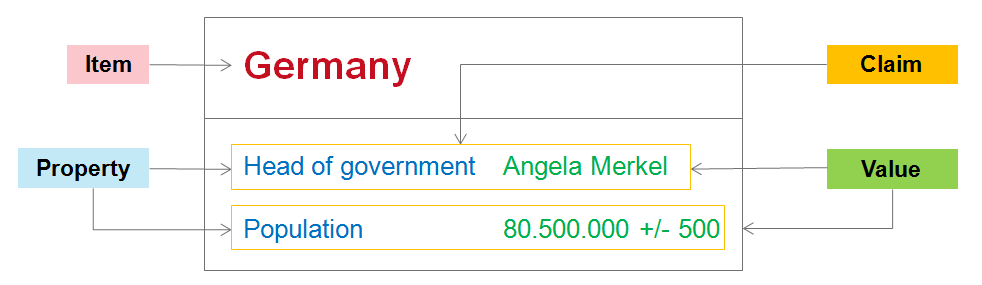
\includegraphics[width=\textwidth]{Pic1}
%\caption{Visualization of claims}
%\label{pic1}
%\end{figure}

Properties can be concretized by qualifiers and a source. A claim under reference to a source is called a "statement". Items and their statements make up the core structure of the data management in Wikidata.

%\begin{figure}[h]
%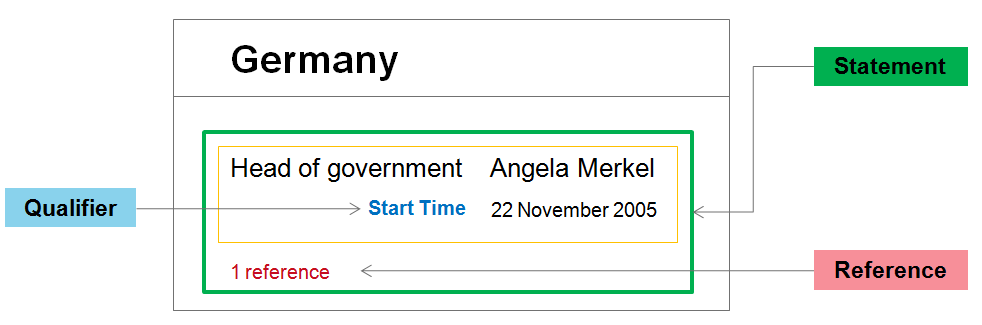
\includegraphics[width=\textwidth]{Pic2}
%\caption{WikiData item}
%\label{pic2}
%\end{figure}

%Items and their statements make up the core structure of the data management in WikiData.

The overall relation between all components can be seen completely in Figure~\ref{pic3} 

\begin{figure}
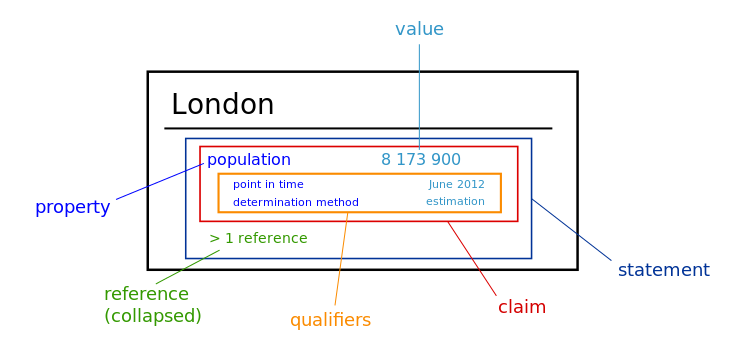
\includegraphics[width=\textwidth]{Pic3}
\caption{Connection between items and statements (Quelle: \url{https://upload.wikimedia.org/wikipedia/commons/thumb/9/98/Wikidata_statement.svg/751px-Wikidata_statement.svg.png})}
\label{pic3}
\end{figure}

\subsection{Data types}
\paragraph{}
WikiData allows data to be modeled from primitive or complex data types. For example, the data type "quantity" is made up of several decimals and an unit:

\begin{itemize}
\item	amount: the quantity's main value
\item	lowerBound: the quantity's lower bound (1 by default)
\item	upperBound: the quantity's upper bound (1 by default)
\item	unit: unit of measure item (empty for dimensionless values)
\end{itemize}

Besides the yearly costs of Berlins new airport, we can also add additional information thanks to the bounds, such as "500.000.000 +/- 50.000.000 Euro". 

There are eight other data types, in total 10 with quantity and mathematical expression, which are already implemented in WikiData:

\textbf{String} is meant for language independent alignment of characters. ISBN and other types of codes belong there.

\textbf{Monolingual text} is used for names, which stays the same in each language. 

\textbf{URL} refers to links directing to external pages such as official web pages and e-mail addresses.

\textbf{Time} is used for all kinds of date and their accuracy. Internally saved in the proleptic Gregorian format, they can be converted and displayed in different formats.

\textbf{Global coordinates} can be pairs of numbers, representing the degree of latitude and longitude or the position relative to a stellar object. The earth is used as the default starting point.

\textbf{Items} is a property, referring to other existing items in WikiData to connect different Wikipedia objects. 

\textbf{Properties} refer similar to Item to other existing properties in Wikidata.

\textbf{Common media} are links to files saved in Wikimedia Commons, like videos or maps.

All data types are separated in two types, depending on how they are saved internally. 

\subsubsection{Value type}
\paragraph{}
The first kind of data types are value types, to which string, time, common media and global coordinates belong to. They have their own data structure, allowing high customization, which enables more advanced methods. Due to that, there is a huge code maintenance overhead, especially for new contributors. 

\subsubsection{Property type}
\paragraph{}
The rest are classified as property types. While they do have their own use cases, they are based on and stored as already existing data types, namely value types. URL and monolingual texts are property types which are based on the string value type. As they share some methods with their parent data type, property types are easy to maintain. While it is also possible to implement advanced methods for these kind of data type, the difficulty and overhead to do so is usually higher then implementing the data type as value type.

\subsection{Data type components}
\paragraph{}
Every data type is made of three components:

\begin{itemize}
\item	Parser: transforms input into a data value
\item	Validator: check data value on additional constrains
\item	Formatter: transforms data value into a fitting output
\end{itemize}
Figure~\ref{pic4} displays the functionality of the components for a given data type:

\begin{figure*}[h]
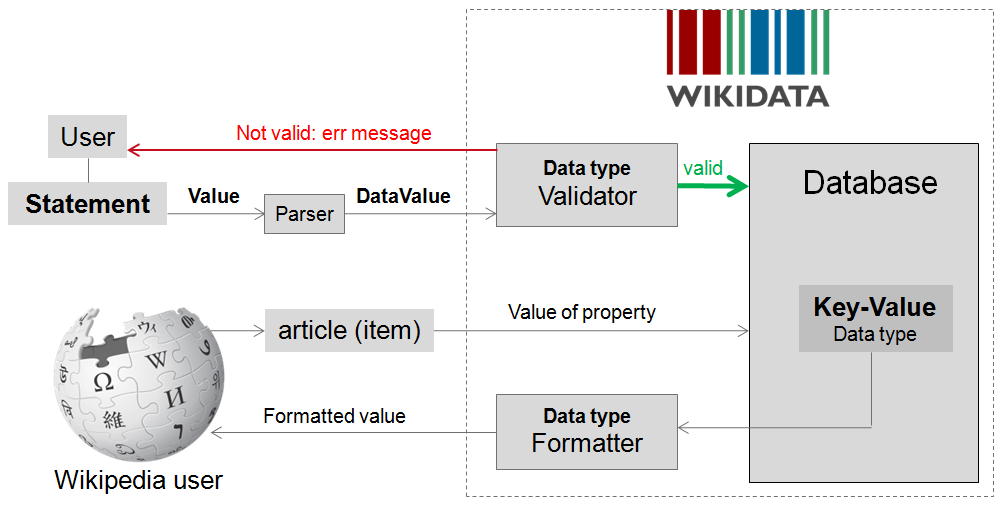
\includegraphics[width=\textwidth]{Pic4}
\caption{Data type components}
\label{pic4}
\end{figure*}

\section{Math formulae}
\paragraph{}
Based on Wikipedia, a formula \textquotedblleft refers to the general construct of a relationship between given quantities [while a math formula] is an entity constructed using the symbols and formation rules of a given logical language."\footnote{https://en.wikipedia.org/wiki/Formula}

Mathematical expressions are currently saved via TeX Strings as pictures in Wikipedia. They are marked and formatted with the \verb|<math>| tag. This Formatting from TeX string to a picture is part of an extention of Wikibase called “Math extension”. It enables the connection between Wikipedia and MathML, which enables formatting of the expression as a readable output for the users. The TeX string \verb|<math>r = \frac{1}{2} d</math>| can be displayed as $r = \frac{1}{2} d$. 

There was no data type in WikiData yet, which could achieve the same display feature as the \verb|<math>| tag. Each formula is embedded in the Wikipedia source, where they were not language independent and had to be added or edited in each language separately. The explanation of parts of the formula also has to be done separately and there wasn't a fixed schemata given to do so. A computer, and maybe even the user, couldn't analyze the formula without text analysis.

\subsection{Necessarily of the data type}
\paragraph{}
An implementation of a new data type for mathematical expression would allow formulae to be
\begin{itemize}
\item	saved language independent and centralized. While the variables might vary in different languages, the meaning of them will always stay the same, which makes a formula language independent.

\item	validated upon input to prevent syntax errors.

\item	formatted given the context it appears. On the one hand, the users can see a formula in a human adjusted output, regardless what kind of browser they use or where they live. On the other hand, while Wikipedia should present a human friendly format, WikiData can provide an output specified for computers.
\end{itemize}

Because of that, there are several options to evolve the usage of formulae. It should be possible to

\begin{itemize}
\item	identify sub-formulae inside the TeX string of a formula with specifications of an item 

\item	have a legend for each formula to interpret them uniform

\item	have queries like "Show me all formulae, where mass is used."
\end{itemize}

%\begin{figure}
%\begin{tabular}{c|c}
%Reasons to implement new data type & Reasons to use given data type\\
%\hline
%\end{tabular}\\
%\end{figure}

Before adding the new data type, we had to make sure whether it's useful enough on its own or another, already existing data type matches our needs. 
Being a language independent information, another option besides implementing an own data type could have been to build an add-on to monolingual text or string though, as it's already used for chemical formula.
%TODO: Maybe you can add a table with pros and cos new datataype vs existing data type I like the example chimical formula very much.
Once added to Wikipedia, a formula usually doesn't change frequently due to being proved by scientist beforehand and checked by certain Wikipedia users afterwards.
Because of the limited scope of targets, the data type will only be relevant for a small portion of Wikipedia.

Mathematical formulae do offer a broader use case as an own data type though. Unlike chemical formulae, mathematical ones have variables and are used for calculations, which can be added to the data type in the future. Something similar is already possible with WolframAlpha\footnote{\url{http://www.wolframalpha.com/}}, a computational knowledge engine which allows the user to enter a formula and returns information such as a graph or zero. It is also possible to use WolframAlpha as a calculator with TeX String as input, a feature which can be build additionally to our data type. While it might be also possible in the add-on idea, it would create a huge overhead for every other use case.

There is no free accessible database containing all kinds of mathematical formulae yet. A separate data type where meta data is stored additionally to the formula enables that. Especially computers can look up all kind or formula way easier.

\section{Implementation choices}
\paragraph{}
Before we could actually start to implement the data type, we had to think about several implementation choices. Because formulae are already displayed in Wikipedia as formatted Tex strings, we decided to keep it like that, because the users, who are already editing the pages, keep a familiar way of editing the information. In general, we had two big choices in implementing the data type: Either creating a new value type "math formulae" or a property type "math formulae" with "string" as value type. Because it would be difficult to change that afterwards without breaking already existing formulae, we had to choose this very early.
In the following, we explain the two options in detail.

\subsection{Math formula as value type}
\paragraph{}
The option of a new value type works similar to geographic coordinates. It would be modeled as a tuple with following elements:
\begin{itemize}
\item The Tex string for displaying the formulae. The general formula for polynomials would be noted as\\ \verb|f(x) = \sum\limits_{i = 0}^{n} a_i x^i|\\
and be displayed in Wikipedia like\\
$f(x) = \sum\limits_{i = 0}^{n} a_i x^i$
\item An array of variables and the link to the respected item they belong to. In this example, $a_i$ would get a link to the item "coefficient"
\item Other meta information as string, regarding the formula. An example would be for a polynomial with degree $n$, the coefficient $a_n$ of $x^n$ is not allowed to be $0$ and $n$ is an element of $\mathds{N}$
\end{itemize}
Combined, the formula could look like this in Wikipedia:\\
$f(x) = \sum\limits_{i = 0}^{n} a_i x^i, n \in \mathds{N}, a_n \neq 0$\\
$a_i$ : coefficient\\
\\
The input for that in WikiData can be equivalent to geographic coordinates:\\
\verb!f(x) = \sum\limits_{i = 0}^{n} a_i x^i;!\\
\verb!a_i : coefficient ;!\\
\verb!n \in \mathds{N}, a_n \neq 0!\\
Each row would represent an element of the tuple.

\subsection{Math formula as property type}
\paragraph{}
Implementing the data type as property type with string as value type would have changed nothing with regards to the output. Instead of storing the information separately in a tuple though, all the information would be in the Tex string. For the example from above, a possible notation would be\\
\verb!f(x) = \sum\limits_{i = 0}^{n} #a_i|coefficient# x^i,!\\ 
\verb!n \in \mathds{N}, a_n \neq 0!\\
On the one hand, we wanted our data type to easily handle complex tasks like easy calculation and linking variables and sub formulae to their respective items, on the other hand we had to make sure that our data type will be usable for Wikipedia users. After a discussion with Lydia Pintscher, the product manager of WikiData, and Daniel Kinzler, a developer from the Wikimedia Foundation, who works on data types in WikiData, we decided to choose the property type version. Maintenance by outsiders is way easier this way and we did not found enough features to justify the overhead the value type implementation would bring.
Before we could start to implement the data type though, we needed something to see how its going to look like when deployed in Wikipedia. 

\section{Test environment}
\paragraph{}
To check, how our implementation will behave when deployed in the production environment, we needed something to simulate WikiData and Wikipedia, as we can't work in the actual WikiData. 
We use a vagrant environment\footnote{\url{https://www.vagrantup.com/}} with wikibase\footnote{\url{https://github.com/wikimedia/mediawiki-extensions-Wikibase}} and math extensions. Vagrant allows us to create our own WikiData environment on a server with the same code used in the actual WikiData with addition to our own one.
It already gave us all the resources we needed and we could work on the same server instead of each of us in a local setup. Because the extensions are also used in WikiData, our implementation will behave very likely in the production environment. To check, how our code would behave in WikiData, we set up a proxy to monitor our outputs\footnote{Link to our main example in our proxy: \url{http://wikidata-math-de.wmflabs.org/wiki/Q10}}.
After we finished to set up our test environment (Figure~\ref{vagrant}), we could start working on our task.

\begin{figure*}[h]
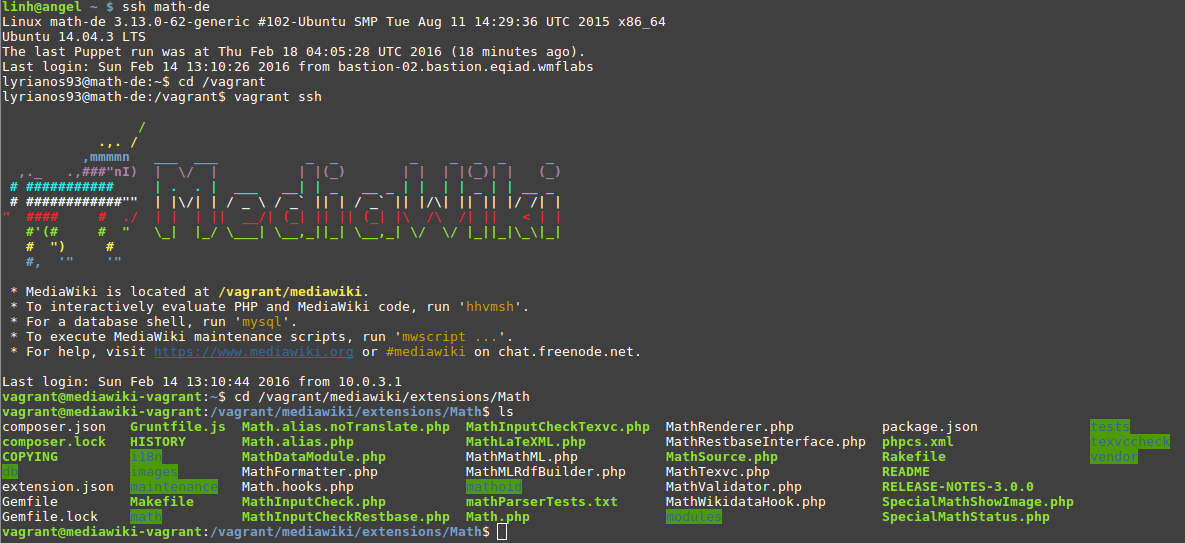
\includegraphics[width = \textwidth]{vagrant}
\caption{Our vagrant environment}
\label{vagrant}
\end{figure*}

\section{Basic implementation}
\paragraph{}
%TODO: Add project gant chart from the presentation.
The implementation process started on the 14th December. 
Following the whole WikiData project, we used php to implement our data type components.
Unlike the other data types, the files for the data type were in the math extension.
Our implementation contains 3 different parts: the hook, the Validator and the Formatter. Usually one has to implement a Parser too. Since we use strings as input method though and use String as value type for our property type implementation, we can simply use the predefined String Parser to transform the input of the user to data values for our Validator and Formatter to process.

The hook (Figure~\ref{hook} at the end of the report) works as the bridge between the math extension via the extension.json\footnote{\url{https://github.com/wikimedia/mediawiki-extensions-Math/blob/master/extension.json}} and the other data types in WikiData. It's the first time, that a new data type is not implemented directly in Wikibase but in an extension. Therefore we needed to set up a hook, which loads the data type within the math extension. It also links the components of the data type and is built similar to the other declarations, calling the respective functions to process the data. There are two declarations, one for the client, which belongs to Wikipedia, and one for the repository, which belongs to WikiData. Unlike the repository, where the information is processed and saved, the client only needs to be able to display the formulae. 

The rdf builder, responsible for additional storage management, was added by another developer.

\begin{figure*}
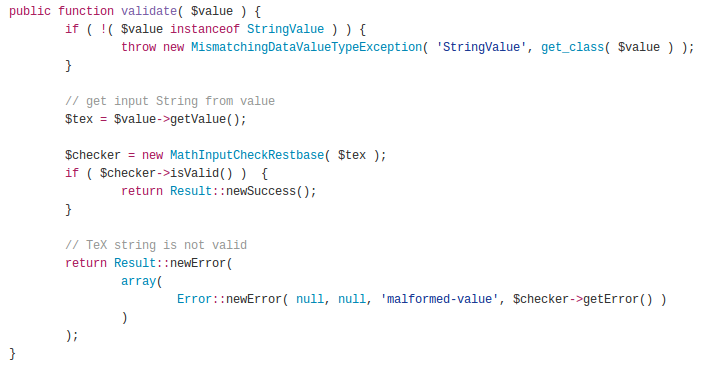
\includegraphics[width = \textwidth]{validate}
\caption{validate function - Validator}
\label{validate}
\end{figure*}
The Validator checks, whether our input is meeting our constrains. At first we check whether our given input is a string value for proper data value transformation.
%TODO List those
The second step is checking if the input is a valid TeX string. This is necessary, because we have to prevent getting an error while formatting the string. In future development, the Validator has to additionally check the meta data, whether they are properly inserted and match the related TeX string.
Once the input passes the Validator, it can be saved in WikiData and later be queried and returned via the Formatter.

The Formatter transforms our Tex string to some kind of output, depending on the use case. It consists of two main functions: construct~\ref{construct} and format~\ref{format}.
\begin{figure*}[h]
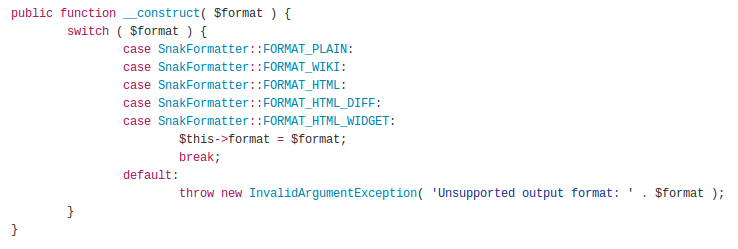
\includegraphics[width = \textwidth]{formatterconstruct}
\caption{construct function - Formatter}
\label{construct}
\end{figure*}

In Wikipedia and WikiData, there are five different output types in total. To ensure our format function can distinguish, which kind of formatting to use, we have to load and store that information via our constructor (Figure~\ref{construct}). Initially, we attempted to include that information directly in the format function, but due to the interface, we couldn't do that. We chose to use Wikibase's  SnakFormatter formats, which can be viewed as a list containing every type of output environment for our Formatter, to have consistent results with the rest of WikiData, although we are taking a higher risk of unpredictable errors, in case the SnakFormatter changes.

\begin{figure*}[h]
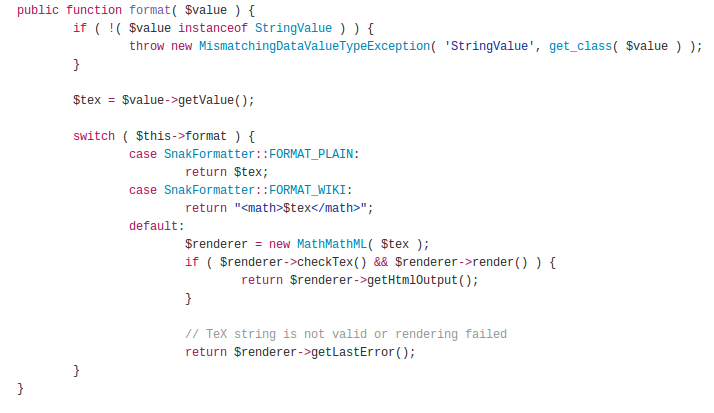
\includegraphics[width = \textwidth]{formatterformat}
\caption{format function - Formatter}
\label{format}
\end{figure*}

Depending on the format loaded in the construct function, the format function (Figure~\ref{format}) processes the TeX string input to resolve that information to a human friendly output.
The plain text is used for input boxes. While it just takes the input, as it is, it also needs to make sure that the input will not be changed.
\begin{figure*}[h]
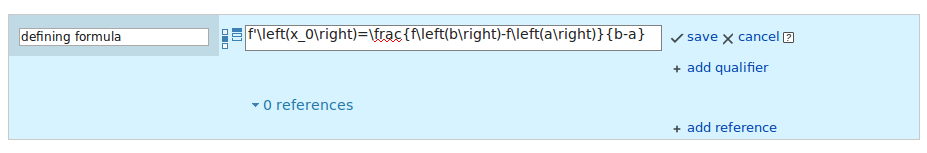
\includegraphics[width = \textwidth]{addValue}
\caption{Adding a value to an item.}
\label{addValue}
\end{figure*}

To display the value in WikiData, it uses HTML output. There are three different kind of HTML outputs, standard HTML for normal output, HTML\_DIFF used in comparison between different versions and HTML\_WIDGET, unknown to us where it is used. We decided to return for each HTML version the processed string, so users can see the result they expect for the Wikipedia article.
\begin{figure*}[h]
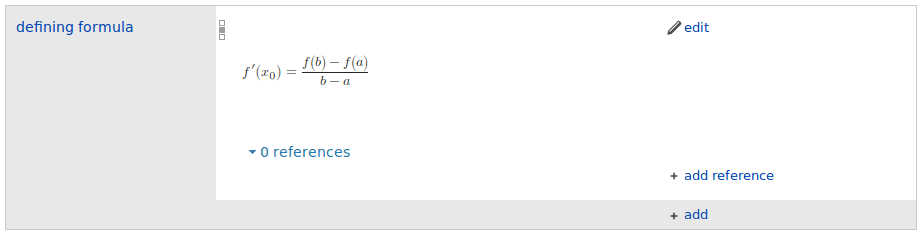
\includegraphics[width = \textwidth]{valueOutput}
\caption{HTML Output in WikiData after formatting the TeX String}
\label{valueOutput}
\end{figure*}

For Wikipedia articles, we use the same output as for HTML but we had to change the way of processing the TeX string because the text in these articles uses another format called x-wiki.
In the future, the format function also need to separate the TeX string and the meta information to create a fitting output.
As we implemented our code, we always had to keep in mind to be able to upgrade our implementation while information added in an early version will have the same output in future versions, namely backwards compatibility.
Our implementation was supposed to merge with the production environment on the 14th January. Because of the review process, it was postponed to the 9th February, which will be explained in the next section.

\section{Testing and developer review}
\paragraph{}
The whole review process regarding our implementation happened on two different platforms, gerrit and phabricator. While gerrit is focused to the code we produced, in phabricator, we discussed everything from the idea to the final product around the implementation\footnote{The whole discussion and everything related about our task can be found at \url{https://phabricator.wikimedia.org/T67397}}.
To ensure that we don't stray off into a wrong path midway, our code was reviewed several times while we worked on it.
Whenever we implemented something, we uploaded it on gerrit\footnote{The review for our implementation can be found at \url{https://gerrit.wikimedia.org/r/\#/c/259167/}}, where our advisor and other Wikimedia developers could review our code and give us feedback. Through several Patch Sets, our code was refined and we were given some ideas, how to improve our code to match the other services in WikiData. One of the comments led to the discussion, whether we want one format function, which internally chose the appropriate format output, or five different Formatter files to keep the code more simple and well separated. We decided to take the single option, as the content wasn't complex enough to separate them, making maintenance and lateral entry easier for other developers. For the Wikipedia user, it wouldn't have changed anything though and if we see the necessity to separate the format function into five.
While working on our basic implementation, we also implement our own tests to check, whether our functions give us the output or error we expect.
Before our implementation was merged into the production environment, it was tested in the beta cluster\footnote{Mainly tested on \url{http://wikidata.beta.wmflabs.org/wiki/Q117940}} of Wikidata.

In the beta cluster, multiple users and developers can check our implementation in an environment closer to the actual Wikipedia and WikiData. At that stage, we had a discussion, how to name the new data type, as some developer thought, "math formula" was to restrictive. That discussion was started due to a missing message, we forgot to implement, because it wasn't necessary in our vagrant environment. In the end, everyone agreed on "Mathematical expression", suggesting more than just relations between entities. The name change caused a bug related with Java Script Caches for some Chrome user though, which caused a delay in the deployment. After we found a solution to the bug, we also had to make sure, no user will be affected by that bug anymore. Our implementation was available to use in the production environment on 9th February.

\section{Community impact}
\paragraph{}
Before the community can start to add formulae as WikiData values, we first need at least one property with the data type Mathematical expression. Because if the dependencies of multiple items to one property, we can't simply add one as WikiData has to make sure, everything stays nice, clean and working. On the one hand, we proposed to change the existing property "Tex string"\footnote{\url{https://www.wikidata.org/wiki/Property:P1993}} from data type string to data type Mathematical expression, on the other hand, we proposed some other properties, such as "defining formula" or "probability density function"\footnote{Both can be found in \url{https://www.wikidata.org/wiki/Wikidata:Property_proposal/Natural_science}}. Both were discussed within the community first before they were actually implemented by certain appropriate user into WikiData.
On 15th February the first property with data type "Mathematical expression" was approved and enabled. On 28th February, 96 items, in the area of math and physics, has a statement with "defining formula" as property. Most of them were added several hours after the announcement of the property being added and the others were added gradually. 

\section{Future development}
\paragraph{}
One question we are facing is where we want to add the meta information in our string.
Adding them in line will result in an intuitive mapping. It will make the string confusing though if there are a lot of them and when there are nested. 
If the meta information is added separately outside the formula, it will make the implementation of the new formatting easier as the user can easily see, how the formula will look like in the end. The downside of that approach will be the huge obstacle the user will face, when trying to edit the formula, depending on how the mapping is implemented.

\newpage

\begin{lstlisting}
class MathWikidataHook {
/**
* Add Datatype "Math" to the Wikibase Repository
*/
public static function onWikibaseRepoDataTypes( array &$dataTypeDefinitions ) {
	global $wgMathEnableWikibaseDataType;
	if ( !$wgMathEnableWikibaseDataType ) {
		return;
	}
	$dataTypeDefinitions['PT:math'] = array(
		'value-type'                 => 'string',
		'validator-factory-callback' => function() {
			// load validator builders
			$factory = WikibaseRepo::getDefaultValidatorBuilders();
			// initialize an array with string validators
			// returns an array of validators
			// that add basic string validation such as preventing empty strings
			$validators = $factory->buildStringValidators();
			$validators[] = new MathValidator();
			return $validators;
		},
		'parser-factory-callback' => function( ParserOptions $options ) {
			$repo = WikibaseRepo::getDefaultInstance();
			$normalizer = new WikibaseStringValueNormalizer( $repo->getStringNormalizer() );
			return new StringParser( $normalizer );
		},
		'formatter-factory-callback' => function( $format, FormatterOptions $options ) {
			global $wgOut;
			$styles = array( 'ext.math.desktop.styles', 'ext.math.scripts', 'ext.math.styles' );
			$wgOut->addModuleStyles( $styles );
			return new MathFormatter( $format );
		},
		'rdf-builder-factory-callback' => function (
			$mode,
			RdfVocabulary $vocab,
			RdfWriter $writer,
			EntityMentionListener $tracker,
			DedupeBag $dedupe
		) {
			return new MathMLRdfBuilder();
		},
	);
}
/*
* Add Datatype "Math" to the Wikibase Client
*/
public static function onWikibaseClientDataTypes( array &$dataTypeDefinitions ) {
	global $wgMathEnableWikibaseDataType;
	if ( !$wgMathEnableWikibaseDataType ) {
		return;
	}
	$dataTypeDefinitions['PT:math'] = array(
		'value-type'                 => 'string',
		'formatter-factory-callback' => function( $format, FormatterOptions $options ) {
			global $wgOut;
			$styles = array( 'ext.math.desktop.styles', 'ext.math.scripts', 'ext.math.styles' );
			$wgOut->addModuleStyles( $styles );
			return new MathFormatter( $format );
		},
	);
}
}
\end{lstlisting}
\begin{figure}[h]
\caption{MathWikidataHook.php}
\label{hook}
\end{figure}


%Literaturverzeichnis
%\bibliographystyle{abbrv}
%\bibliography{bibliography}
\end{document}